% =============================================================================
% 10-file-organization-hashing-notes.tex — Lecture Notes for Week 10:
% One Probe (File Organization & Hashing)
%
% DERIVED ARTIFACT. Source of truth:
% Slides/CS301/10-file-organization-hashing.tex (54 pp incl. title/transitions).
% Generated by /lecture-notes at the "textbook-candidate prose" Detail Bar
% (every trace step written out, every example fully solved, Exercises with a
% separate Solutions block, reading guidance per section); do not hand-edit
% content independently of the Beamer source without re-running /qa-notes
% afterward (single-source-of-truth.md).
%
% Page-grounding (inherited 1:1 from the deck header; no upgrades):
%   Sedgewick2011 Sec.3.4 (Hash Tables, p.458, section start only);
%   Wirth2004 Sec.5.1 Introduction p.177, Sec.5.2 Choice of a Hash Function
%   p.177, Sec.5.3 Collision Handling p.178, Sec.5.4 Analysis of Key
%   Transformation p.180; Karumanchi2017 Ch.14 (Hashing, pp.610-639 PDF).
%   Horowitz & Sahni Ch.8 (file organization) and Aho-Hopcroft-Ullman Ch.4
%   (hashing) are chapter-level only — no page numbers are asserted.
%   All six TikZ diagrams are reused verbatim from the deck.
%
% Compile with (macOS/Linux, ':'-joined TEXINPUTS/BIBINPUTS): cd Notes/CS301 &&
%   TEXINPUTS=../../Preambles:$TEXINPUTS xelatex -interaction=nonstopmode 10-file-organization-hashing-notes.tex
%   BIBINPUTS=../..:$BIBINPUTS bibtex 10-file-organization-hashing-notes
%   TEXINPUTS=../../Preambles:$TEXINPUTS xelatex -interaction=nonstopmode 10-file-organization-hashing-notes.tex  (x2)
% =============================================================================

\documentclass[11pt]{article}
\usepackage[margin=1in]{geometry}
% =============================================================================
% Preambles/header.tex — shared LaTeX/Beamer preamble for this project
%
% Use from a Beamer lecture by prepending:
%     \input{header}
% and compiling with TEXINPUTS=../Preambles:$TEXINPUTS (the /compile-latex
% skill does this automatically).
%
% PALETTE CONTRACT. Color names defined here MUST match the names in
% Quarto/theme-template.scss so Beamer and Quarto renderings use the same
% palette. The scripts/check-palette-sync.sh script enforces this.
%
% To customize: edit the HEX values below AND the matching $variable in
% Quarto/theme-template.scss, then run scripts/check-palette-sync.sh.
% =============================================================================

% -----------------------------------------------------------------------------
% Engine detection + encoding
%
% Our /compile-latex skill uses XeLaTeX, where inputenc is unnecessary and
% can produce encoding warnings. Only load inputenc under pdfTeX.
% -----------------------------------------------------------------------------
\usepackage{iftex}
\ifPDFTeX
  \usepackage[utf8]{inputenc}
\fi

\usepackage{amsmath, amssymb, amsthm}
\usepackage{booktabs}
\usepackage{graphicx}

% -----------------------------------------------------------------------------
% PALETTE — mirrors Quarto/theme-template.scss variable names.
% Load xcolor and define colors BEFORE anything that references them
% (notably hyperref, hypersetup, and the Beamer color assignments).
% -----------------------------------------------------------------------------
\usepackage{xcolor}

\definecolor{primary-blue}{HTML}{012169}      % headings, accents
\definecolor{primary-gold}{HTML}{B9975B}      % emphasis, borders
\definecolor{highlight-yellow}{HTML}{F2A900}  % markers, alerts
\definecolor{light-bg}{HTML}{E8EDF5}          % title / section backgrounds
\definecolor{jet}{HTML}{1A1A1A}               % body text

% Semantic colors (used in diagrams and annotations)
\definecolor{positive}{HTML}{15803D}          % good / observed / identified
\definecolor{negative}{HTML}{B91C1C}          % bad / problematic / bias
\definecolor{neutral}{HTML}{525252}           % reference / context

% Highlight accents (match .hi-* classes in the SCSS)
\definecolor{hi-slate}{HTML}{314F4F}
\definecolor{hi-green}{HTML}{2E8B57}
\definecolor{hi-red}{HTML}{C41E3A}

% Semantic aliases so skill templates and snippets can write
% \textcolor{accent}{...} without hard-coding "primary-blue".
\colorlet{accent}{primary-blue}
\colorlet{accent2}{primary-gold}

% -----------------------------------------------------------------------------
% Hyperref — loaded AFTER xcolor + palette so link colors resolve.
% -----------------------------------------------------------------------------
\usepackage{hyperref}
\hypersetup{colorlinks=true, linkcolor=primary-blue, urlcolor=primary-blue,
            citecolor=primary-blue, pdfborder={0 0 0}}

% -----------------------------------------------------------------------------
% Course code — set once per deck (after \input{header}, before \begin{document})
% via \coursecode{CS401}. Shown in the footer on every slide so a deck's course
% is identifiable without opening the title page. Empty by default.
% -----------------------------------------------------------------------------
\makeatletter
\newcommand{\coursecode}[1]{\gdef\@coursecodetext{#1}}
\gdef\@coursecodetext{}
\makeatother

% -----------------------------------------------------------------------------
% Beamer theme assignments (only apply under Beamer).
%
% We detect Beamer via \@ifclassloaded{beamer}, which is the documented,
% non-internal way. This must be wrapped in \makeatletter/\makeatother
% because \@ifclassloaded contains an @-catcode character.
% -----------------------------------------------------------------------------
\makeatletter
\@ifclassloaded{beamer}{%
  \usefonttheme{professionalfonts}
  \setbeamercolor{structure}{fg=primary-blue}
  \setbeamercolor{frametitle}{fg=primary-blue}
  \setbeamercolor{title}{fg=primary-blue}
  \setbeamercolor{subtitle}{fg=primary-gold}
  \setbeamercolor{author}{fg=primary-blue}
  \setbeamercolor{institute}{fg=neutral}
  \setbeamercolor{date}{fg=primary-gold}
  \setbeamercolor{itemize item}{fg=primary-blue}
  \setbeamercolor{itemize subitem}{fg=primary-gold}
  \setbeamercolor{alerted text}{fg=primary-gold}
  \setbeamercolor{block title}{fg=white, bg=primary-blue}
  \setbeamercolor{block body}{bg=light-bg}
  % Semantic block variants: block=definition/concept (blue), exampleblock=
  % worked example (green/positive), alertblock=key takeaway or caution (gold).
  % Keep to <=2 colored boxes per slide across ALL three variants (INV-7).
  \setbeamercolor{block title example}{fg=white, bg=positive}
  \setbeamercolor{block body example}{bg=light-bg}
  \setbeamercolor{block title alerted}{fg=white, bg=primary-gold}
  \setbeamercolor{block body alerted}{bg=light-bg}

  % Minimal footer: course code (left) + page X / N (right), no navigation clutter
  \setbeamertemplate{navigation symbols}{}
  \setbeamertemplate{footline}{%
    \color{neutral}\footnotesize\hspace{0.7em}\@coursecodetext\hfill
    \insertframenumber/\inserttotalframenumber\hspace{0.7em}\vspace{0.3em}}
}{}
\makeatother

% -----------------------------------------------------------------------------
% TikZ setup — libraries the snippet gallery uses
% -----------------------------------------------------------------------------
\usepackage{tikz}
\usetikzlibrary{arrows.meta, positioning, calc, decorations.pathreplacing,
                fit, shapes.geometric, backgrounds}

% Shared TikZ styles — snippets and hand-written diagrams can pick these up
% via `\begin{tikzpicture}[every node/.style={...}]` or by naming specific
% styles (e.g., `\node[dag-node] (X) at (0,0) {X};`).
\tikzset{
  % Node styles for causal DAGs and similar
  dag-node/.style = {
    draw=primary-blue, fill=light-bg, rounded corners=2pt,
    minimum width=1.2cm, minimum height=0.9cm, align=center, font=\small
  },
  decision-node/.style = {
    draw=primary-gold, fill=white, diamond, aspect=1.8,
    minimum width=1.8cm, minimum height=1.2cm, align=center, font=\small,
    inner sep=1pt
  },
  % Edge styles — observed vs counterfactual
  observed-edge/.style = {-{Latex[length=2.5mm]}, thick, draw=jet},
  counterfactual-edge/.style = {-{Latex[length=2.5mm]}, thick, draw=neutral, dashed},
  confound-edge/.style = {-{Latex[length=2.5mm]}, thick, draw=negative, dashed},
  % Data-point styles for plots
  observed-dot/.style = {fill=primary-blue, draw=primary-blue, circle, inner sep=1.2pt},
  counterfactual-dot/.style = {fill=white, draw=neutral, circle, inner sep=1.2pt}
}

% -----------------------------------------------------------------------------
% Convenience macros
% -----------------------------------------------------------------------------
\newcommand{\muted}[1]{\textcolor{neutral}{#1}}
\newcommand{\key}[1]{\textcolor{primary-gold}{\textbf{#1}}}
\newcommand{\good}[1]{\textcolor{positive}{#1}}
\newcommand{\bad}[1]{\textcolor{negative}{#1}}

% Standout frame macro: full-bleed dark background for section transitions.
% Beamer-only (uses \begin{frame}/\setbeamercolor/\usebeamerfont) -- do not
% call from an article-class file (e.g. Notes/<CODE>/*-notes.tex). \muted,
% \key, \good, \bad, and \coursecode above are plain xcolor/gdef and are
% safe to use from either class; verified when Notes/article-class support
% was added.
% Expand: \transitionslide{Your transition title}
\newcommand{\transitionslide}[1]{%
  \begingroup
  \setbeamercolor{background canvas}{bg=primary-blue}
  \begin{frame}[plain]
    \centering
    \vfill
    {\usebeamerfont{title}\color{white}\Large #1\par}
    \vfill
  \end{frame}
  \endgroup
}

% Section divider frame (Beamer-only), an alternative to \transitionslide with a
% darker two-line style: near-black (jet) background, a small white label line
% above a larger gold title, and a thin gold rule along the bottom edge.
% Expand: \sectiondivider{Section 2}{Pointers}
\newcommand{\sectiondivider}[2]{%
  \begingroup
  \setbeamercolor{background canvas}{bg=jet}
  \begin{frame}[plain]
    \vspace*{3.0cm}
    {\color{white}\ttfamily\large #1\par}
    \vspace{0.5cm}
    {\color{primary-gold}\LARGE #2\par}
    \begin{tikzpicture}[remember picture, overlay]
      \draw[primary-gold, line width=2.5pt]
        ($(current page.south west)+(0,0.1)$) -- ($(current page.south east)+(0,0.1)$);
    \end{tikzpicture}
  \end{frame}
  \endgroup
}

% -----------------------------------------------------------------------------
% Channel watermark — "Concepts That Click" (YouTube).
%
% Article-class files (CompetitiveExam Q/A sets, Notes, Assignments) get a
% light diagonal draft watermark on every page plus a centered footer naming
% the channel. Beamer decks get a subtle TikZ background watermark instead
% (the footline already carries the course code). Centralized here so every
% MCQ PDF is branded without per-file edits.
% -----------------------------------------------------------------------------
\makeatletter
\@ifclassloaded{article}{%
  \usepackage{draftwatermark}
  \SetWatermarkText{Concepts That Click}
  \SetWatermarkScale{1}
  \SetWatermarkFontSize{2cm}
  \SetWatermarkLightness{0.86}
  \SetWatermarkAngle{45}
  \usepackage{fancyhdr}
  \pagestyle{fancy}
  \fancyhf{}
  \fancyfoot[C]{\footnotesize\textcolor{neutral}{Concepts That Click~|~YouTube: \href{https://www.youtube.com/@concepts.thatclick}{@concepts.thatclick}}}
  \renewcommand{\headrulewidth}{0pt}
  \renewcommand{\footrulewidth}{0pt}
  \fancypagestyle{plain}{%
    \fancyhf{}%
    \fancyfoot[C]{\footnotesize\textcolor{neutral}{Concepts That Click~|~YouTube: \href{https://www.youtube.com/@concepts.thatclick}{@concepts.thatclick}}}%
    \renewcommand{\headrulewidth}{0pt}%
    \renewcommand{\footrulewidth}{0pt}%
  }
}{}
\@ifclassloaded{beamer}{%
  \setbeamertemplate{background}{%
    \begin{tikzpicture}[remember picture, overlay]
      \node[rotate=45, opacity=0.055, align=center]
        at (current page.center)
        {\Huge\textcolor{neutral}{Concepts That Click}};
    \end{tikzpicture}%
  }
}{}
\makeatother 
\coursecode{CS301}

% Emergency stretch so long \texttt{} tokens in prose do not spill the margin.
\setlength{\emergencystretch}{2.5em}

% Chapter-style numbering: this is Week 10's chapter.
\renewcommand{\thesection}{10.\arabic{section}}
\renewcommand{\thefigure}{10.\arabic{figure}}
\newtheorem{example}{Example}[section]

\newenvironment{definitionbox}[1]{%
  \par\noindent\textbf{Definition (#1).}\ \itshape
}{\par\vspace{0.3em}}

\title{One Probe\\\large Lecture Notes --- Week 10: File Organization \& Hashing}
\author{Auqib Hamid Lone\\[0.3em]
  \small Department of Computer Science \& Engineering\\
  \small Government College of Engineering \& Technology (GCET), Ganderbal}
\date{\today}

\begin{document}
\maketitle

\section{Why This Week Exists: One Probe}

\textbf{Read alongside:} Sedgewick, \textit{Algorithms}, Sec.~3.4, p.458 --- hash tables as the third symbol-table implementation; Karumanchi, \textit{Data Structures and Algorithms Made Easy}, Ch.~14, pp.610--639 (PDF) --- the hash-table ADT, load factor, and collision resolution.

Week~9 ended with the calculator's $2{,}000$-identifier table sorted in $\Theta(n\log n)$, searched by binary search in about $\log_2 2{,}000 \approx 11$ comparisons, and it closed on a promise: \emph{can we find a record in one probe, without sorting at all?} This chapter pays that promise off. It does not re-teach the linked list (Week~6), the sorted array and binary search (Weeks~8--9), or the address arithmetic that turns an index into a location (Week~3); it uses all three.

The deficiency is not search speed --- eleven comparisons is excellent --- but the \emph{insert}. A sorted array must keep its order, so adding one new identifier shifts every record that sorts after it: $\Theta(n)$ per insert, and the tokenizer can insert thousands of names. Hashing removes the order, and with it the shifting.

The deck's five questions organize the chapter. How should records be laid out in a file so that one can be found without scanning the rest? What makes a hash function \emph{good}, and what makes one silently bad? Two keys want the same slot: what are the two families of fixes, and why are their names backwards? Why does a hash table promise $O(1)$ yet degrade to $O(n)$? When should a designer refuse hashing and keep order instead?

The bill for a lookup is the table below. The counts are probes (or comparisons of keys), not CPU instructions, and the hash row assumes a load factor of $\alpha = n/m = 0.5$.

\begin{center}
{\footnotesize
\begin{tabular}{l r l}
  \toprule
  \textbf{structure for 2{,}000 identifiers} & \textbf{probes} & \textbf{insert} \\
  \midrule
  unsorted linked list (Week 6) & $\approx 1{,}000$ & $O(1)$ at head \\
  sorted array $+$ binary search (Weeks 8--9) & $\approx 11$ & $\Theta(n)$ \\
  hash table (this week, $\alpha = 0.5$) & $\approx 1.25$ & $O(1)$ expected \\
  \bottomrule
\end{tabular}}
\end{center}

The sorted array bought a factor of about $1{,}000/11 \approx 91$ by \emph{ordering} the data. The hash table buys a further factor of about $11/1.25 \approx 9$ by \emph{abandoning} order, and the chapter must say what that costs: a hash table cannot answer ``the next key'' or ``every key between $a$ and $b$''. The hash table does not search for the key at all. It computes where the key must be, then checks that one place:
\[
  \text{slot} = h(\text{key}).
\]
Everything else in the chapter --- collisions, probing, deletion, resizing --- is the price of making that one line of arithmetic work on real keys.

\muted{Running application (Weeks 3--11): one calculator, rebuilt each week. Week 10 replaces its identifier list with a hash table --- the same $2{,}000$ names, now found in one or two probes instead of a thousand.}

\section{Files, Records, and Access Schemes}

\textbf{Read alongside:} Wirth, \textit{Algorithms and Data Structures}, Sec.~5.1, p.177 --- the introduction to key transformations and why a computed address replaces a search; Horowitz \& Sahni, \textit{Fundamentals of Data Structures}, Ch.~8 (standard treatment) --- file organization, sequential and direct files.

\begin{definitionbox}{record, field, key \cite{HorowitzSahni2008_fundamentals_data_structures}}
A \key{record} is a fixed-length collection of fields describing one entity. One field is designated the \key{key}: its value identifies the record and is the only part a search compares. A \key{file} is a collection of records stored on a device.
\end{definitionbox}

A concrete record is a student's $64$-byte entry \texttt{\{roll, name[40], programme, year, marks\}}, keyed by \texttt{roll}. The key is not always unique: names repeat. A \key{primary key} is unique and identifies at most one record; a \key{secondary key} is not unique and may index many records. Every organization in this section answers one question --- given a key, how many device reads occur before the record is in memory? --- and the answer is counted in \emph{block transfers}, not CPU instructions.

Four access schemes describe how a device is used. They are properties of the device and the layout, not of the algorithm: a tape cannot do direct access, and a disk pays for every seek.

\begin{center}
{\footnotesize
\begin{tabular}{l p{5.0cm} p{4.6cm}}
  \toprule
  \textbf{access scheme} & \textbf{how the device is used} & \textbf{typical medium} \\
  \midrule
  serial & read every record from the beginning & magnetic tape \\
  sequential & read the next record, in stored order & tape, sorted file \\
  direct (random) & seek straight to a computed block & disk, SSD \\
  indexed & look up a key in an index, then seek & disk, database \\
  \bottomrule
\end{tabular}}
\end{center}

The file organizations that follow are four ways of combining these access schemes with a record layout. Their costs differ by orders of magnitude, and the difference is entirely in how many blocks the device must deliver.

\section{Four File Organizations}

\textbf{Read alongside:} Horowitz \& Sahni, Ch.~8 (standard treatment) --- sequential, direct, and indexed file organization; Wirth, Sec.~5.1, p.177 --- the move from a searched address to a computed one.

\subsection{Sequential files: the pile and the sorted file}

Records are stored one after another, either in the order they arrive (a \key{pile}) or in key order (a \key{sorted sequential} file).

In an unsorted pile, search is $\Theta(n)$: scan until the key appears, or until the file ends. Insert is $\Theta(1)$: append at the end. Delete is $\Theta(n)$ if the gap must be closed by shifting later records, or $\Theta(1)$ with a mark bit that leaves a dead record in place.

In a sorted sequential file, the picture splits by device. On a tape, search is still a linear scan, because a tape cannot jump. On a direct-access device, fixed-length records make the $j$-th record reachable by arithmetic, so binary search works and costs $\Theta(\log n)$ seeks. Insert and delete become $\Theta(n)$: every later record must shift to keep the order.

\begin{example}
A file holds $1{,}000$ student records of $64$ bytes each. Finding the last record in an unsorted sequential file costs up to $1{,}000$ reads --- every record is touched. Sorting the file makes a fixed-length binary search possible: $\lceil\log_2 1000\rceil = 10$ seeks, since $2^9 = 512 < 1000 \le 1024 = 2^{10}$. But inserting one student now moves every record after the insertion point, which is $\Theta(n)$ record rewrites. The order that made search cheap made insert expensive.
\end{example}

Sequential organization wins exactly where the workload reads every record anyway --- payroll runs, end-of-term processing --- and where the data is too large for any index to help.

\subsection{Direct (relative) files: the address is computed}

A direct file removes the search entirely. The record's location is computed from its key:
\[
  \text{offset} = (\text{key} - k_0)\times L,
  \qquad
  \text{address} = \text{base} + \text{offset},
\]
where $k_0$ is the smallest key in the file and $L$ is the record length in bytes. Search, insert and delete are all $\Theta(1)$: one seek, one write, no comparison.

The catch is the key space. Keys must be dense integers, because the offset formula reserves one slot for every integer between $k_0$ and the largest key. A file for employee numbers $\{1, 7, 100{,}000\}$ would need $100{,}000$ slots to store three records.

\begin{example}
Roll numbers run from $20230001$ to $20231000$, with records of $64$ bytes. Roll $20230457$ has relative record number $457 - 1 = 456$, so it sits at offset
\[
  456 \times 64 = 29{,}184 \text{ bytes}
\]
from the base of the file. One seek, no search at all. This is the ideal that hashing will imitate for arbitrary keys: replace the constant $k_0$ and the multiplier $L$ with a function $h$ that accepts any key.
\end{example}

\begin{figure}[h]
  \centering
  % Diagram: key -> relative record number -> byte offset -> one seek.
  % Four boxes at y=0, x-centres 0, 2.7, 4.9, 7.4. Arrow labels sit above
  % the arrows, never on them.
  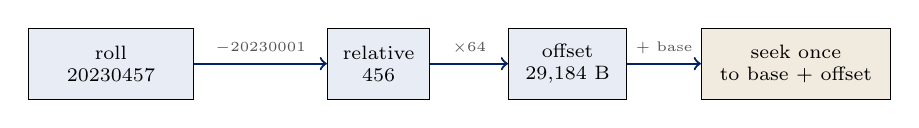
\begin{tikzpicture}[every node/.style={font=\scriptsize}]
    \node[draw, fill=light-bg, minimum width=2.1cm, minimum height=0.9cm,
      align=center] (k) at (0, 0) {roll\\ $20230457$};
    \node[draw, fill=light-bg, minimum width=1.3cm, minimum height=0.9cm,
      align=center] (r) at (3.4, 0) {relative\\ $456$};
    \node[draw, fill=light-bg, minimum width=1.5cm, minimum height=0.9cm,
      align=center] (o) at (5.8, 0) {offset\\ $29{,}184$ B};
    \node[draw, fill=primary-gold!20, minimum width=2.4cm,
      minimum height=0.9cm, align=center] (a) at (8.7, 0) {seek once\\ to base $+$ offset};
    \draw[->, thick, primary-blue] (k) -- (r)
      node[midway, above, text=neutral] {\tiny $-20230001$};
    \draw[->, thick, primary-blue] (r) -- (o)
      node[midway, above, text=neutral] {\tiny $\times 64$};
    \draw[->, thick, primary-blue] (o) -- (a)
      node[midway, above, text=neutral] {\tiny $+$ base};
  \end{tikzpicture}
  \caption{The direct file as one arithmetic pipeline: subtract the first key, multiply by the record length, add the base address, seek once --- cf.\ \textit{Horowitz \& Sahni}, Ch.~8 (standard treatment) \cite{HorowitzSahni2008_fundamentals_data_structures}.}
  \label{fig:direct}
\end{figure}

The whole organization is a single arithmetic pipeline, shown in Figure~\ref{fig:direct}. It works until the key space is sparse --- which is the normal case for names, account numbers and arbitrary identifiers, and the reason a general hash function is needed.

\subsection{Indexed sequential files}

An indexed sequential file keeps the data file sorted by key but stores it in \emph{blocks}, and builds a sparse \key{index} with one entry per block: that block's highest key and its address. The index is small enough to be searched quickly, and each index entry covers many records.

Search binary-searches the index for the block, then scans that block. With $B$ blocks of $b$ records each, the cost is $\Theta(\log B + b)$ reads: a logarithmic search over block boundaries, then a linear scan inside one block. Insert places the record in its correct block if there is room, and otherwise in an \key{overflow area} that the index still reaches; a periodic \key{reorganization} merges the overflow back into the main file and rebuilds the index.

Indexed sequential wins when the workload needs point lookups \emph{and} ordered or range scans. It is the classic ISAM organization, and the shape that a B-tree index generalizes in Week~12's databases.

\subsection{Hashed files: replacing the search with arithmetic}

A hashed file generalizes the direct file to arbitrary keys. Instead of deriving the address from a dense key, it computes the bucket address:
\[
  \text{bucket} = h(\text{key}) \bmod m,
  \qquad \text{read that bucket, then search inside it.}
\]
If two keys hash to the same bucket, the bucket holds more than one record --- an \key{overflow chain}. The bucket, not the record, is the unit of one device read.

\begin{definitionbox}{hashed file \cite{Sedgewick2011_algorithms}}
A file whose record address is $h(\text{key})$; collisions are resolved by chaining or by probing. It supports point queries, not range queries.
\end{definitionbox}

Search is expected $\Theta(1)$ when the buckets are short, and order is gone: there is no ``next record in key order''. Every remaining section is about making $h$ good and keeping the buckets short without destroying the $\Theta(1)$ promise.

\subsection{The four organizations side by side}

\begin{center}
{\footnotesize\setlength{\tabcolsep}{4pt}
\begin{tabular}{p{2.9cm} p{2.0cm} p{2.0cm} p{2.6cm} p{2.3cm}}
  \toprule
  \textbf{organization} & \textbf{search} & \textbf{insert} &
    \textbf{range scan} & \textbf{extra space} \\
  \midrule
  sequential (pile) & $\Theta(n)$ & $\Theta(1)$ & $\Theta(n)$ & none \\
  sequential (sorted) & $\Theta(\log n)$ seeks & $\Theta(n)$ &
    $\Theta(n)$ & none \\
  direct / relative & $\Theta(1)$ & $\Theta(1)$ & $\Theta(\text{range})$ &
    key range \\
  indexed sequential & $\Theta(\log B + b)$ & overflow $+$ reorg &
    $\Theta(\log B + \text{out})$ & index $+$ overflow \\
  hashed & $\Theta(1)$ expected & $\Theta(1)$ expected &
    $\Theta(n+m)$ (no order) & table $+$ chain \\
  \bottomrule
\end{tabular}}
\end{center}

Read the table by \emph{which column is fast}. Hashing wins the first two columns and loses the third; indexed sequential is the only one strong in both. The choice is a workload question, exactly as it was for sorting in Week~9. A hashed file, in short, is an array we never search.

\section{The Hash-Table ADT and the Load Factor}

\textbf{Read alongside:} Sedgewick, Sec.~3.4, p.458 --- the hash-table API and the load-factor analysis; Wirth, Sec.~5.1, p.177 and Sec.~5.2, p.177 --- choice of a hash function; Aho--Hopcroft--Ullman, Ch.~4 (standard treatment) --- hash functions and collision resolution.

\begin{definitionbox}{hash table \cite{Sedgewick2011_algorithms,Wirth2004_algorithms_data_structures}}
A hash table stores $n$ keys in $m$ slots. A \key{hash function} $h: U \to \{0,\dots,m-1\}$ maps each key to a slot. It supports \texttt{insert}, \texttt{search} and \texttt{delete}; the \key{load factor} is $\alpha = n/m$.
\end{definitionbox}

Collisions are unavoidable. The universe $U$ is larger than $m$, so by the pigeonhole principle two keys must share a slot. The design question is not how to prevent this but what to do when it happens.

The cost model is the \emph{expected number of probes} under \key{uniform hashing}: each key is equally likely to hash to any slot, independently of the others. Every formula in this chapter is an expectation under that assumption, which is why a hash function that is biased on the \emph{actual} keys invalidates all of them.

The table does not store keys in order. \texttt{search} is fast; \texttt{min}, \texttt{max} and ``all keys between $a$ and $b$'' are not supported at all.

\begin{example}
The calculator's symbol table holds $n = 2{,}000$ identifiers. Choosing $\alpha = n/m = 0.5$ fixes the table size:
\[
  m = \frac{n}{\alpha} = \frac{2{,}000}{0.5} = 4{,}000 \text{ slots}.
\]
Under separate chaining the expected successful-search cost is $1 + \alpha/2 = 1.25$ comparisons, and the expected unsuccessful cost is $\alpha = 0.5$. Compare the sorted array's $11$ comparisons and the unsorted list's $\approx 1{,}000$. The table is not magic: it bought its speed by spending $4{,}000$ slots on $2{,}000$ keys, and by giving up order.
\end{example}

\subsection{What makes a good hash function}

Four properties decide whether a function is usable.

\textbf{Deterministic.} The same key must always hash to the same slot, or a stored record can never be found again. Determinism is not a performance property; without it the structure is incorrect.

\textbf{Uniform.} Over the keys actually used, the outputs should spread evenly over the $m$ slots. A function that is uniform on random keys but biased on real keys is a bad function. This is the property that the load-factor formulas silently assume.

\textbf{Fast.} Computing $h$ must cost less than the search it replaces. A cryptographic hash is uniform but far too slow for a symbol table: the point is to save comparisons, not to spend more work hashing than searching would have cost.

\textbf{Uses the whole key.} If the table size is $m = 2^p$, then $h(k) = k \bmod m$ sees only the low $p$ bits. Two keys differing only in high bits collide every time. Any function that ignores part of the key has thrown away the information that distinguishes those keys.

The test that matters is the one a textbook cannot supply: hash the \emph{actual} key distribution. Student roll numbers share a year prefix, employee numbers share a company prefix, names share letters. A good $h$ must break those patterns, and the only way to know whether it does is to run it on a sample of real keys and count the bucket lengths.

\section{Designing the Hash Function}

\textbf{Read alongside:} Wirth, Sec.~5.2, p.177 --- choice of a hash function; Sedgewick, Sec.~3.4, p.458 --- modular hashing and its table-size requirements; Karumanchi, Ch.~14, pp.610--639 (PDF) --- division, mid-square, folding and string hash functions.

\subsection{The division method}

The simplest method, and the fastest, is
\[
  h(k) = k \bmod m.
\]
The only design decision is $m$, and it matters more than the formula suggests. Choose $m$ \key{prime}, preferably not close to a power of $2$ or $10$; then every digit of $k$ can affect the residue.

Why not $m = 2^p$? Because $k \bmod 2^p$ is exactly the low $p$ bits of $k$: even keys use only half the slots, and sequential keys give sequential residues. Why not $m = 10^p$? Because decimal keys share trailing zeros, so the residue simply repeats the key's pattern rather than mixing it.

\begin{example}
Take $m = 11$ and compute the residues directly:
\[
  \begin{aligned}
    12 &= 1\cdot 11 + 1 &&\Rightarrow h(12) = 1,\\
    44 &= 4\cdot 11 + 0 &&\Rightarrow h(44) = 0,\\
    88 &= 8\cdot 11 + 0 &&\Rightarrow h(88) = 0,\\
    23 &= 2\cdot 11 + 1 &&\Rightarrow h(23) = 1,\\
    94 &= 8\cdot 11 + 6 &&\Rightarrow h(94) = 6.
  \end{aligned}
\]
Two collisions already: $44$ and $88$ both want slot $0$, and $12$ and $23$ both want slot $1$. The arithmetic is not failing --- it is doing exactly what a map from a large universe to eleven slots must do. The next two sections are entirely about handling these collisions.
\end{example}

\begin{figure}[h]
  \centering
  % Diagram: four keys enter h(k)=k mod 11; three slots lie to the right.
  % Key boxes at x=0, y = 1.5, 0.7, -0.1, -0.9; function box centred at
  % (2.3,0.3); slots at x=4.9, y = 1.0, 0.2, -0.6.
  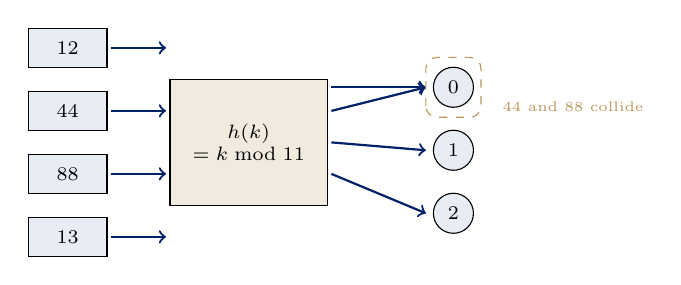
\begin{tikzpicture}[every node/.style={font=\scriptsize}]
    \foreach \y/\v in {1.5/12, 0.7/44, -0.1/88, -0.9/13}
      \node[draw, fill=light-bg, minimum width=1.0cm,
        minimum height=0.5cm] at (0, \y) {\v};
    \node[draw, fill=primary-gold!20, minimum width=2.0cm,
      minimum height=1.6cm, align=center] (h) at (2.3, 0.3)
      {$h(k)$\\ $=k \bmod 11$};
    \foreach \y in {1.5, 0.7, -0.1, -0.9}
      \draw[->, thick, primary-blue] (0.55, \y) -- (1.25, \y);
    \foreach \y/\v in {1.0/0, 0.2/1, -0.6/2}
      \node[draw, circle, fill=light-bg, inner sep=3pt] at (4.9, \y) {\v};
    \draw[->, thick, primary-blue] (3.35, 1.0) -- (4.55, 1.0);
    \draw[->, thick, primary-blue] (3.35, 0.7) -- (4.55, 1.0);
    \draw[->, thick, primary-blue] (3.35, 0.3) -- (4.55, 0.2);
    \draw[->, thick, primary-blue] (3.35, -0.1) -- (4.55, -0.6);
    \draw[dashed, primary-gold, rounded corners]
      (4.55, 0.62) rectangle (5.25, 1.38);
    \node[text=primary-gold, anchor=west] at (5.4, 0.75)
      {\tiny $44$ and $88$ collide};
  \end{tikzpicture}
  \caption{Four keys through $h(k)=k \bmod 11$: $12\mapsto 1$, $44\mapsto 0$, $88\mapsto 0$, $13\mapsto 2$. The collision at slot $0$ is the function behaving as defined, not a fault --- cf.\ \textit{Sedgewick}, Sec.~3.4, p.458 \cite{Sedgewick2011_algorithms}.}
  \label{fig:hashmap}
\end{figure}

Figure~\ref{fig:hashmap} draws the map as a map: four keys in, three slots out, and the collision at slot $0$ is the arithmetic working as defined.

\subsection{The multiplication method}

The multiplication method avoids the choice of a prime:
\[
  h(k) = \left\lfloor m\,(kA \bmod 1)\right\rfloor,
  \qquad 0 < A < 1.
\]
Multiply the key by a fixed fraction $A$, keep the fractional part, and scale it to $m$ slots. Knuth's choice is
\[
  A = \frac{\sqrt{5}-1}{2} \approx 0.6180339887,
\]
the golden-ratio conjugate.

The advantage is that $m$ need not be prime and is often a power of two, so the scaling becomes a shift rather than a division. The method uses the \emph{high} bits of the product, so it does not ignore the key's leading digits --- precisely the failure mode of the division method with $m = 2^p$. The cost is one multiplication and a fractional-part extraction: still constant time, slightly more work than a division.

\begin{example}
Take $m = 16$ and Knuth's $A = 0.6180339887$. For $k = 12{,}345$,
\[
  kA = 12{,}345 \times 0.6180339887 = 7{,}629.6296\ldots
\]
The integer part is $7{,}629$; the fractional part is $0.6296\ldots$. Scaling to sixteen slots,
\[
  h(k) = \lfloor 16 \times 0.6296\ldots\rfloor = \lfloor 10.07\ldots\rfloor = 10.
\]
The low bits of $k$ did not decide the slot; the product did. An implementation fixes $A$ once at full precision and uses that exact value, because the fractional part is sensitive to the constant.
\end{example}

\subsection{The classic four}

\begin{center}
{\footnotesize
\begin{tabular}{l l p{5.4cm}}
  \toprule
  \textbf{method} & \textbf{formula} & \textbf{note} \\
  \midrule
  division & $k \bmod m$ & choose prime $m$; fast; the default \\
  multiplication & $\lfloor m(kA \bmod 1)\rfloor$ &
    any $m$; uses high bits; Knuth's $A$ \\
  mid-square & middle digits of $k^2$ &
    key digits influence all output digits \\
  folding & add or XOR the key's parts &
    good for fixed-width records and IDs \\
  digit analysis & choose the most uniform digits &
    needs a sample of real keys \\
  \bottomrule
\end{tabular}}
\end{center}

\textbf{Mid-square.} Square the key and take the middle digits, so that every digit of the key can influence every digit of the hash. For $k = 5678$,
\[
  k^2 = 32{,}239{,}684,
\]
and the middle four digits of the eight-digit square are $2396$. The leading and trailing digits are discarded because they are the least mixed: the leading digits depend only on the high part of $k$, the trailing digits only on the low part.

\textbf{Folding.} Split the key into fixed-width parts and add them, optionally with carries ignored or with XOR. For $123456789$,
\[
  123 + 456 + 789 = 1368,
\]
and $1368 \bmod m$ is the slot. This suits fixed-width records and identifiers whose digits carry positional meaning.

\textbf{Digit analysis.} Examine a sample of real keys and choose the digits that vary most. If every roll number begins $2023$, those four digits carry no information and should be dropped; hash the remainder. This method is the only one on the list that requires knowledge of the data, which is exactly why it can outperform the arithmetic methods on real keys.

\subsection{Hashing strings}

Keys are usually strings, not integers. Treat a string as a polynomial in a base $B$ and evaluate it modulo $m$ by Horner's rule:
\[
  h(s) = \Bigl(\cdots\bigl((s_0 B + s_1)B + s_2\bigr)\cdots\Bigr) \bmod m.
\]
$B = 31$ is the common choice: small, prime, and cheap to multiply by a shift and a subtract ($31x = 32x - x$).

In C, the running value must be reduced modulo $m$ at every step. A $32$-bit \texttt{unsigned} overflows once $31^n$ exceeds $2^{32}$, which happens after about seven characters; the reduction inside the loop is what keeps the arithmetic well defined. Use unsigned arithmetic so the intermediate products wrap predictably rather than invoking signed overflow.

\begin{example}
Hash \texttt{"cat"} with $m = 97$ and $B = 31$. The character codes are \texttt{'c'}$=99$, \texttt{'a'}$=97$, \texttt{'t'}$=116$. Start with $h = 0$:
\[
  \begin{aligned}
    h &= 0\cdot 31 + 99 &&= 99,\\
    h &= 99\cdot 31 + 97 &&= 3{,}069 + 97 = 3{,}166,\\
    h &= 3{,}166\cdot 31 + 116 &&= 98{,}146 + 116 = 98{,}262.
  \end{aligned}
\]
Finally $98{,}262 = 97 \times 1{,}013 + 1$, so $h(\texttt{"cat"}) = 1$. Reducing at each step instead of at the end gives the same answer, because reduction modulo $m$ commutes with addition and multiplication.
\end{example}

\subsection{Universal hashing}

A fixed $h$ can always be defeated. An adversary who knows the function can choose keys that all collide --- for a symbol table fed by untrusted input, that is a denial-of-service waiting to happen. The defence is to choose the function \emph{randomly at table creation} from a family, and to keep the choice secret from the input.

\begin{definitionbox}{universal family \cite{AhoHopcroftUllman1983_data_structures_algorithms}}
Let $p$ be a prime larger than the key universe, and choose $a \in \{1,\dots,p-1\}$ and $b \in \{0,\dots,p-1\}$ uniformly at random. Then
\[
  h_{a,b}(k) = \bigl((ak+b) \bmod p\bigr) \bmod m
\]
satisfies $\Pr[h_{a,b}(k_1) = h_{a,b}(k_2)] \le 1/m$ for every distinct $k_1, k_2$.
\end{definitionbox}

The probability bound is what makes the guarantee uniform: no fixed input can force a bad distribution, because the function is not fixed until after the adversary has committed to the keys. The expected cost is $O(1+\alpha)$ over the random choice. Libraries use this whenever keys are attacker-controlled.

\subsection{A bad hash function, traced}

Suppose the key is a student's year of admission followed by a sequence number, and we hash with $m = 100$ by taking the last two digits. Sequential IDs spread perfectly over the hundred slots, and that is fine. The same function fails as soon as the key distribution changes.

Take $m = 10$ and suppose every key is even: $20230002, 20230004, \dots, 20230040$. Then
\[
  k \bmod 10 \in \{0,2,4,6,8\},
\]
so five of the ten slots are never used. With $20$ keys the nominal load factor is $\alpha = 20/10 = 2$, but the load on the five usable slots is $20/5 = 4 = 2\alpha$. Every formula in this chapter that is stated in terms of $\alpha$ now understates the cost by a factor of two at least.

The second failure is subtler. Take $m = 2^{10} = 1024$ and a cohort whose keys differ only in the high-order year bits. The remainder keeps only the low $10$ bits, so every student in the cohort collides in the same few slots --- the table is nearly empty and the chains are long at the same time.

\begin{example}
A concrete trace of the first failure. Hash the twenty even keys $20230002$ through $20230040$ with $m = 10$:
\[
  \begin{array}{c|cccccccccc}
    \text{slot} & 0 & 1 & 2 & 3 & 4 & 5 & 6 & 7 & 8 & 9\\
    \hline
    \text{keys} & 4 & 0 & 4 & 0 & 4 & 0 & 4 & 0 & 4 & 0
  \end{array}
\]
Five slots hold four keys each and five hold none. The average chain over \emph{usable} slots is $4$, while $\alpha$ reports $2$. Changing $m$ to $11$ or $13$ removes the pattern, because a prime modulus lets the odd and even positions of the key mix.
\end{example}

The rule of thumb follows: a hash function is only as good as its behaviour on the keys you will actually store. Test it on a sample, count the bucket lengths, and look at the longest chain. If one bucket holds a large fraction of $n$, change $m$ or change $h$ --- do not blame the collision policy for a distribution the function created.

\section{Open Hashing: Separate Chaining}

\textbf{Read alongside:} Wirth, Sec.~5.3, p.178 --- collision handling by chaining and by probing; Sedgewick, Sec.~3.4, p.458 --- separate chaining and its analysis; Karumanchi, Ch.~14, pp.610--639 (PDF) --- the chaining implementation.

\subsection{Two names, one warning}

The terminology is historically confusing, and an unqualified name is ambiguous on an exam. Two keys can want the same slot; that is normal, not an error, and the two families of fixes below differ only in where the second key goes.

\begin{definitionbox}{open hashing / closed hashing \cite{Wirth2004_algorithms_data_structures}}
\key{Open hashing} is \key{separate chaining}: colliding keys are stored \emph{outside} the table, in a list attached to the slot. \key{Closed hashing} is \key{open addressing}: every key is stored \emph{inside} the table, and collisions are resolved by probing other slots.
\end{definitionbox}

``Open'' refers to the table being open to an unbounded number of entries per slot. ``Closed'' refers to the address space being closed: a key must end up in one of the $m$ slots. The syllabus uses both pairs, so whenever either name appears, give the alternative in the same sentence.

\subsection{The idea}

The table is an array of $m$ \key{heads}. Slot $j$ points to a linked list of every key with $h(k) = j$.

Insert computes $h(k)$ and pushes the key onto that slot's list, in $\Theta(1)$. This is Week~6's linked list, one per bucket. Search computes $h(k)$, then walks that one list comparing keys; the list is short if $h$ is uniform. Delete unlinks the node --- $\Theta(1)$ after the search, with no tombstones and no probing. The load factor $\alpha = n/m$ can exceed $1$: the table has $m$ slots but no limit on the total number of nodes.

\begin{figure}[h]
  \centering
  % Diagram: m=11 buckets. Non-empty chains only:
  % 0: 44->88->11, 1: 12->23, 2: 13, 5: 16->5, 6: 94->39, 9: 20.
  % Heads at y=-0.85, deeper nodes at -1.6 and -2.35; n=11, alpha=1.0.
  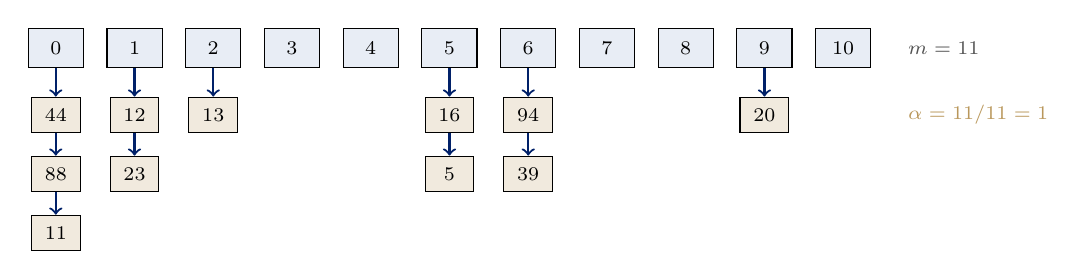
\begin{tikzpicture}[every node/.style={font=\scriptsize}]
    \foreach \i in {0,...,10}
      \node[draw, fill=light-bg, minimum width=0.7cm,
        minimum height=0.5cm] (b\i) at (\i, 0) {\i};
    \foreach \i/\v in {0/44, 1/12, 2/13, 5/16, 6/94, 9/20}
      \node[draw, fill=primary-gold!20, minimum width=0.62cm,
        minimum height=0.45cm] (h\i) at (\i, -0.85) {\v};
    \foreach \i in {0,1,2,5,6,9}
      \draw[->, thick, primary-blue] (b\i) -- (h\i);
    \node[draw, fill=primary-gold!20, minimum width=0.62cm,
      minimum height=0.45cm] (s0) at (0, -1.6) {88};
    \node[draw, fill=primary-gold!20, minimum width=0.62cm,
      minimum height=0.45cm] (s1) at (1, -1.6) {23};
    \node[draw, fill=primary-gold!20, minimum width=0.62cm,
      minimum height=0.45cm] (s5) at (5, -1.6) {5};
    \node[draw, fill=primary-gold!20, minimum width=0.62cm,
      minimum height=0.45cm] (s6) at (6, -1.6) {39};
    \node[draw, fill=primary-gold!20, minimum width=0.62cm,
      minimum height=0.45cm] (t0) at (0, -2.35) {11};
    \foreach \a/\b in {h0/s0, h1/s1, h5/s5, h6/s6, s0/t0}
      \draw[->, thick, primary-blue] (\a) -- (\b);
    \node[text=neutral, anchor=west] at (10.7, 0)
      {$m=11$};
    \node[text=primary-gold, anchor=west] at (10.7, -0.85)
      {$\alpha=11/11=1$};
  \end{tikzpicture}
  \caption{Separate chaining with $m=11$: each bucket owns a head and a list. Slot $0$'s chain holds three keys and slot $1$'s two; empty buckets have no chain. The trace below follows $h(k)=k \bmod 11$ exactly --- cf.\ \textit{Sedgewick}, Sec.~3.4, p.458, and \textit{Wirth}, Sec.~5.3, p.178 \cite{Sedgewick2011_algorithms,Wirth2004_algorithms_data_structures}.}
  \label{fig:chaining}
\end{figure}

Figure~\ref{fig:chaining} shows the shape of the structure: an array of heads, each pointing into a list of nodes. For the traces that follow, take the eleven keys $12, 44, 13, 88, 23, 94, 11, 39, 20, 16, 5$ inserted under $h(k) = k \bmod 11$. Computing the residues,
\[
  \begin{array}{c|ccccccccccc}
    k & 12 & 44 & 13 & 88 & 23 & 94 & 11 & 39 & 20 & 16 & 5\\
    \hline
    h(k) & 1 & 0 & 2 & 0 & 1 & 6 & 0 & 6 & 9 & 5 & 5
  \end{array}
\]
so the chains are
\[
  \begin{array}{c|l}
    \text{slot} & \text{chain (walk order)}\\
    \hline
    0 & 44 \to 88 \to 11\\
    1 & 12 \to 23\\
    2 & 13\\
    5 & 16 \to 5\\
    6 & 94 \to 39\\
    9 & 20
  \end{array}
\]
Six buckets are occupied and five are empty. The lists are drawn in walk order, which is the only order a chain search uses.

\begin{example}
\textbf{Search $23$.} Compute $h(23) = 1$. Read head $1$: compare $12$ (no), follow the link, compare $23$ (yes). Two comparisons, independent of the other ten keys.

\textbf{Search $50$, a miss.} Compute $h(50) = 50 - 44 = 6$. Walk slot $6$'s chain: $94$, then $39$, then the null pointer. Two comparisons, and the miss is detected without scanning the rest of the table. A miss costs the whole chain; a hit costs on average half of it.
\end{example}

\begin{example}
\textbf{Insert $60$.} Compute $h(60) = 5$ (since $55 \le 60 < 66$). Push at the head of slot $5$: the chain $16 \to 5$ becomes
\[
  60 \to 16 \to 5.
\]
One pointer write, one increment of $n$. No key is moved, no slot is reprobed, and no other bucket is touched.

\textbf{Delete $88$.} Search slot $0$'s chain for $88$: $44$ (no), $88$ (yes) --- the second node. Unlink it by redirecting the predecessor's pointer:
\[
  44 \to 88 \to 11 \quad\longrightarrow\quad 44 \to 11.
\]
The other two nodes of the chain keep their positions and no other slot is disturbed. This is Week~6's pointer surgery, and it is the one operation where chaining is unambiguously simpler than open addressing: there is no tombstone to leave behind and no probe sequence to preserve.
\end{example}

\subsection{The bill}

Under uniform hashing, the expected number of key comparisons in a chain is
\[
  \text{successful} \approx 1 + \frac{\alpha}{2},
  \qquad
  \text{unsuccessful} \approx \alpha.
\]
The successful cost is half the chain because the target is equally likely to be anywhere in it; the leading $1$ is the comparison that succeeds. The unsuccessful cost is the whole chain, because a miss examines every node.

\begin{center}
{\footnotesize
\begin{tabular}{r r r}
  \toprule
  $\alpha = n/m$ & successful & unsuccessful \\
  \midrule
  $0.5$ & $1.25$ & $0.5$ \\
  $1.0$ & $1.5$  & $1.0$ \\
  $2.0$ & $2.0$  & $2.0$ \\
  $4.0$ & $3.0$  & $4.0$ \\
  \bottomrule
\end{tabular}}
\end{center}

Space is $\Theta(n+m)$: $n$ nodes plus $m$ heads. Chaining degrades gracefully --- doubling $n$ doubles the cost rather than squaring it --- which is why a chained table can be allowed to run at $\alpha > 1$ and then resized.

\begin{verbatim}
typedef struct Entry {
    const char *key; int value; struct Entry *next;
} Entry;
typedef struct { Entry **head; int m; int n; } Table;

unsigned hash(const char *s, int m) {
    unsigned h = 0;
    for (; *s; s++) h = (h * 31u + (unsigned char)*s) % (unsigned)m;
    return h;
}
int table_search(Table *t, const char *key, int *out) {
    Entry *e = t->head[hash(key, t->m)];
    for (; e; e = e->next)
        if (!strcmp(e->key, key)) { if (out) *out = e->value; return 1; }
    return 0;
}
int table_insert(Table *t, const char *key, int value);  /* push at head */
\end{verbatim}

Insert links one \texttt{Entry} at the head and increments \texttt{n}. Resize --- allocate $2m$ heads, rehash every node --- when $\alpha > 1$. The \texttt{hash} function is the polynomial string hash of the previous section with $B = 31$, reduced at every step; \texttt{table\_search} is a single chain walk, which is exactly the two-comparison trace above with a general \texttt{m}.

\section{Closed Hashing: Open Addressing}

\textbf{Read alongside:} Wirth, Sec.~5.3, p.178 and Sec.~5.4, p.180 --- collision handling and the analysis of key transformation; Sedgewick, Sec.~3.4, p.458 --- linear probing, clustering and double hashing; Karumanchi, Ch.~14, pp.610--639 (PDF) --- open addressing.

\subsection{The idea}

Open addressing stores every key \emph{in the table}. There are no pointers, no nodes and no allocation --- just an array of $m$ slots. On a collision it follows a \key{probe sequence}
\[
  h(k),\; h(k)+1,\; h(k)+2,\; \dots \pmod m
\]
until an empty slot is found. Search follows the same sequence until the key is found or an \emph{empty} slot proves it absent. Delete must leave a marker, because clearing a slot would destroy that proof.

The load factor is $\alpha = n/m \le 1$ by construction. Performance is controlled by keeping $\alpha$ below a threshold ($0.5$--$0.75$) and rehashing when it is exceeded. The structure is cache-friendly: the probe sequence walks contiguous memory, which is why open addressing often beats chaining in wall-clock time even at the same asymptotic cost.

\subsection{Linear probing}

The simplest probe sequence is
\[
  h(k,i) = \bigl(h'(k) + i\bigr) \bmod m, \qquad i = 0,1,2,\dots
\]
Insert probes $h'(k), h'(k)+1, \dots$ until an empty slot; search makes the same walk until it finds the key or an empty slot.

\begin{example}
Take $m = 11$, $h'(k) = k \bmod 11$, and insert $12, 44, 13, 88, 23, 94$ in that order. Each insert is written out in full.

\textbf{Insert $12$.} $h'(12) = 1$; slot $1$ is empty, so $12$ goes to slot $1$ with one probe.

\textbf{Insert $44$.} $h'(44) = 0$; slot $0$ is empty, so $44$ goes to slot $0$ with one probe.

\textbf{Insert $13$.} $h'(13) = 2$; slot $2$ is empty, so $13$ goes to slot $2$ with one probe.

\textbf{Insert $88$.} $h'(88) = 0$. Slot $0$ holds $44$ (occupied), slot $1$ holds $12$ (occupied), slot $2$ holds $13$ (occupied), slot $3$ is empty. Four probes; $88$ lands at slot $3$.

\textbf{Insert $23$.} $h'(23) = 1$. Slot $1$ holds $12$, slot $2$ holds $13$, slot $3$ now holds $88$, slot $4$ is empty. Four probes; $23$ lands at slot $4$.

\textbf{Insert $94$.} $h'(94) = 6$; slot $6$ is empty, so $94$ goes to slot $6$ with one probe.

The final table is
\[
  \begin{array}{c|ccccccccccc}
    \text{slot} & 0 & 1 & 2 & 3 & 4 & 5 & 6 & 7 & 8 & 9 & 10\\
    \hline
    \text{key} & 44 & 12 & 13 & 88 & 23 & \cdot & 94 & \cdot & \cdot & \cdot & \cdot
  \end{array}
\]
The two keys that were displaced from their home slots are $88$ and $23$, and each paid four probes to be placed.
\end{example}

\begin{figure}[h]
  \centering
  % Diagram: final 11-slot table after inserting 12,44,13,88,23,94.
  % Slots at x=0..10, y=0. The brace below slots 1..4 marks the four probes
  % made by search(23); the brace is 0.55 cm below the slot boxes.
  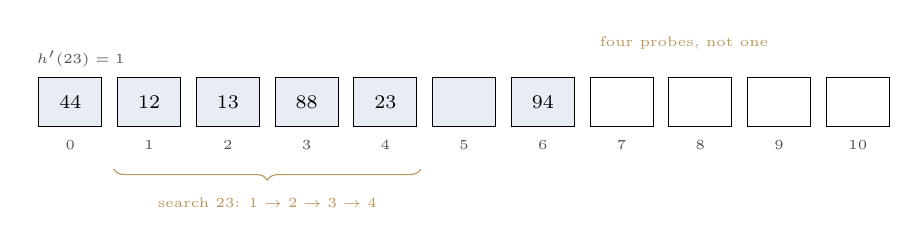
\begin{tikzpicture}[every node/.style={font=\scriptsize}]
    \foreach \i/\v in {0/44, 1/12, 2/13, 3/88, 4/23, 5/{}, 6/94}
      \node[draw, fill=light-bg, minimum width=0.8cm,
        minimum height=0.62cm] at (\i, 0) {\v};
    \foreach \i/\v in {7/{}, 8/{}, 9/{}, 10/{}}
      \node[draw, fill=white, minimum width=0.8cm,
        minimum height=0.62cm] at (\i, 0) {\v};
    \foreach \i in {0,...,10}
      \node[text=neutral] at (\i, -0.55) {\tiny \i};
    \draw[decorate, decoration={brace, mirror, amplitude=4pt},
      primary-gold] (0.55, -0.85) -- (4.45, -0.85)
      node[midway, below=7pt, text=primary-gold]
      {\tiny search $23$: $1 \to 2 \to 3 \to 4$};
    \node[text=neutral, anchor=west] at (-0.55, 0.55) {%
      \tiny $h'(23)=1$};
    \node[text=primary-gold, anchor=west] at (6.6, 0.75)
      {\tiny four probes, not one};
  \end{tikzpicture}
  \caption{The table after six linear-probing inserts. Searching for $23$ walks slots $1,2,3,4$ --- four probes, because $88$ and $23$ were displaced into a run --- cf.\ \textit{Sedgewick}, Sec.~3.4, p.458 \cite{Sedgewick2011_algorithms}.}
  \label{fig:linear}
\end{figure}

The collision has been paid for by every later search, not just by the insert: finding $23$ costs four probes, shown by the brace in Figure~\ref{fig:linear}, even though one probe would have sufficed in an empty table.

\begin{example}
Predict the next insert before reading on. The table holds $44$ at slot $0$, $12$ at slot $1$, $13$ at slot $2$, $88$ at slot $3$, $23$ at slot $4$ and $94$ at slot $6$; slots $5$ and $7$--$10$ are empty. Insert $11$, whose home slot is $h'(11) = 0$.

The probe visits slot $0$ ($44$), slot $1$ ($12$), slot $2$ ($13$), slot $3$ ($88$), slot $4$ ($23$) --- all occupied --- and lands at slot $5$, the first empty slot. One insert paid five probes.

A search for $11$ now makes six comparisons, slots $0$ through $5$. The cost of the insert has become the cost of every later lookup of that key. That is the difference between linear probing and a chain: the chain's insert touches one node, while the probe's insert commits every future search to the same walk.
\end{example}

Insert cost is paid once; probe cost is paid on every search. The rest of the section is about keeping both small.

\subsection{Primary clustering}

Once a run of occupied slots forms, any key that hashes into the run must traverse the whole run and extend it. Runs grow faster than the keys that created them --- this is \key{primary clustering}. Knuth's expected probe counts for linear probing are
\[
  \text{successful} \approx \frac12\left(1+\frac{1}{1-\alpha}\right),
  \qquad
  \text{unsuccessful} \approx \frac12\left(1+\frac{1}{(1-\alpha)^2}\right).
\]

\begin{center}
{\footnotesize
\begin{tabular}{r r r}
  \toprule
  $\alpha$ & successful & unsuccessful \\
  \midrule
  $0.25$ & $1.17$ & $1.39$ \\
  $0.50$ & $1.50$ & $2.50$ \\
  $0.75$ & $2.50$ & $8.50$ \\
  $0.90$ & $5.50$ & $50.5$ \\
  $0.95$ & $10.5$ & $200.5$ \\
  \bottomrule
\end{tabular}}
\end{center}

The formulas are worth checking at one point. At $\alpha = 0.5$, the successful cost is $\frac12(1 + 1/0.5) = \frac12(1+2) = 1.5$, and the unsuccessful cost is $\frac12(1 + 1/0.25) = \frac12(5) = 2.5$. The unsuccessful column is the warning: at $\alpha = 0.9$ a miss costs about $50$ probes, and at $\alpha = 0.95$ about $200$. Linear probing is safe only well below $0.75$.

\subsection{Deletion: the tombstone}

Delete $13$ from slot $2$ of the trace. If the slot is simply cleared, a later search for $88$ probes slot $0$ (occupied by $44$), slot $1$ (occupied by $12$), slot $2$ (\emph{empty}) --- and concludes that $88$ is absent. It is wrong: $88$ sits at slot $3$, one slot past the hole.

The empty slot is the search's stopping condition, so deletion must not create one. Mark the slot \key{DELETED} --- a \key{tombstone}. Search treats \texttt{DELETED} as occupied and continues. Insert may reuse the first tombstone it meets. When tombstones dominate, rebuild the table (\key{rehash}), because a table full of tombstones has the probe cost of a full table without the keys.

\begin{example}
Delete $13$ from the six-key table of the previous example, using $m = 11$ and $h'(k) = k \bmod 11$.

The search for $13$ starts at slot $2$, finds it immediately, and writes \texttt{DELETED} into slot $2$. The table is now $44$ at $0$, $12$ at $1$, \texttt{DELETED} at $2$, $88$ at $3$, $23$ at $4$, $94$ at $6$.

Now search for $88$. $h'(88) = 0$: slot $0$ holds $44$ (not it, continue), slot $1$ holds $12$ (not it, continue), slot $2$ holds \texttt{DELETED} (not it, \emph{keep going} --- this is the whole point), slot $3$ holds $88$ (found). Four probes.

If slot $2$ had been cleared to \texttt{EMPTY}, the same search would stop at slot $2$ and report that $88$ is absent. The key would still be in the table and would be unreachable --- a correctness bug, not a slowdown. One tombstone converts a successful search into a false miss.
\end{example}

\begin{figure}[h]
  \centering
  % Diagram: slots 0..4 after deleting 13. Search(88) must pass 0,1,2,3.
  % Slot 2 is DELETED (red dashed); the probing path is a brace below.
  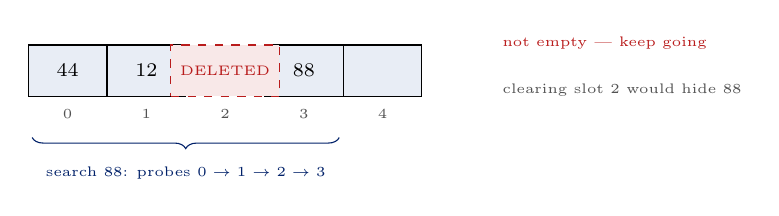
\begin{tikzpicture}[every node/.style={font=\scriptsize}]
    \foreach \i/\v in {0/44, 1/12, 3/88, 4/{}}
      \node[draw, fill=light-bg, minimum width=1.0cm,
        minimum height=0.65cm] at (\i, 0) {\v};
    \node[draw=negative, fill=negative!10, dashed, text=negative,
      minimum width=1.0cm, minimum height=0.65cm, align=center]
      at (2, 0) {\tiny DELETED};
    \foreach \i in {0,...,4}
      \node[text=neutral] at (\i, -0.55) {\tiny \i};
    \draw[decorate, decoration={brace, mirror, amplitude=4pt},
      primary-blue] (-0.45, -0.85) -- (3.45, -0.85)
      node[midway, below=7pt, text=primary-blue]
      {\tiny search $88$: probes $0 \to 1 \to 2 \to 3$};
    \node[text=negative, anchor=west] at (5.4, 0.35)
      {\tiny not empty --- keep going};
    \node[text=neutral, anchor=west] at (5.4, -0.25)
      {\tiny clearing slot $2$ would hide $88$};
  \end{tikzpicture}
  \caption{After deleting $13$, slot $2$ must read \texttt{DELETED}, not empty. The search for $88$ passes through the tombstone and continues to slot $3$ --- cf.\ \textit{Wirth}, Sec.~5.3, p.178 \cite{Wirth2004_algorithms_data_structures}.}
  \label{fig:tombstone}
\end{figure}

The tombstone is a promise: ``a key may have passed through here.'' Every slot therefore has one of three states, not two --- \texttt{EMPTY} stops a search, \texttt{DELETED} does not --- and that extra state is the closed-hashing price for having no pointers. Figure~\ref{fig:tombstone} draws the three states together.

\subsection{Quadratic probing}

Quadratic probing changes the step so that a key does not simply extend a run:
\[
  h(k,i) = \bigl(h'(k) + c_1 i + c_2 i^2\bigr) \bmod m.
\]
The probe offsets are $0,\; c_1+c_2,\; 2c_1+4c_2,\; \dots$ --- not consecutive. It removes \emph{primary} clustering but creates \key{secondary clustering}: keys with the same home slot follow the same sequence, so they still collide with each other, just not with the neighbours of the run.

The reachability guarantee is subtler than linear probing's. With $m$ prime and offsets $i^2$ (that is, $c_1 = 0$, $c_2 = 1$), only $\lceil m/2\rceil$ slots are reachable, so keep $\alpha \le 1/2$. With $m = 2^p$ and offsets $i(i+1)/2$, all slots are reachable. Expected probes are lower than linear at the same $\alpha$, but the arithmetic is more expensive and the cache behaviour is worse.

\begin{example}
Take $m = 11$, $h'(k) = k \bmod 11$, and offsets $c_1 = 0$, $c_2 = 1$, so the probe sequence for a key is $h', h'+1, h'+4, h'+9, \dots$ modulo $11$. For $k = 23$, $h'(23) = 1$, and the probes are
\[
  1,\quad (1+1)=2,\quad (1+4)=5,\quad (1+9)=10,
\]
that is, slots $1, 2, 5, 10$. Slot $1$ is the home slot; the next three probes jump by $1$, $3$ and $5$. The key never touches slots $3$ or $4$, so it does not extend the run that $88$ and $23$ created under linear probing.
\end{example}

\subsection{Double hashing}

Double hashing makes the step size a second hash of the key:
\[
  h(k,i) = \bigl(h_1(k) + i\,h_2(k)\bigr) \bmod m.
\]
Two keys with the same home slot usually take different paths, which makes this the closest practical approximation to uniform hashing. The requirement is that $h_2(k)$ be \key{coprime to $m$}, or the sequence visits only a fraction of the slots. With prime $m$, choose $h_2(k) \in \{1,\dots,m-1\}$; with $m = 2^p$, force $h_2(k)$ odd. A common choice is
\[
  h_2(k) = 1 + (k \bmod (m-1)),
\]
which is never $0$ and is coprime to a prime $m$.

\begin{example}
Take $m = 11$, $h_1(k) = k \bmod 11$, and $h_2(k) = 1 + (k \bmod 10)$. For $k = 23$:
\[
  h_1(23) = 1, \qquad h_2(23) = 1 + (23 \bmod 10) = 1 + 3 = 4.
\]
The probe sequence adds $4$ each time, modulo $11$:
\[
  1,\; 5,\; 9,\; (9+4)\bmod 11 = 2,\; 6,\; 10,\; 3,\; 7,\; 0,\; 4,\; 8.
\]
That is eleven distinct slots --- every slot exactly once --- because $\gcd(4,11) = 1$. Had $h_2(23)$ been $0$, the sequence would have been stuck at slot $1$; had it shared a factor with $m$, the walk would have visited only a subset.
\end{example}

\begin{figure}[h]
  \centering
  % Diagram: probe order for key 23 (h1=1) under the three schemes.
  % Rows at y=2.2 (linear), 0.8 (quadratic), -0.6 (double); slots x=0..10.
  % Filled slots carry the probe number 1..4.
  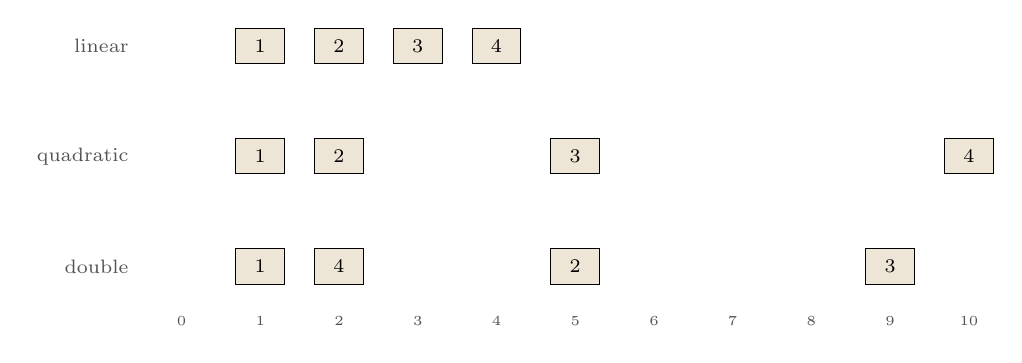
\begin{tikzpicture}[every node/.style={font=\scriptsize}]
    \foreach \r/\lab in {2.2/linear, 0.8/quadratic, -0.6/double}
      \node[text=neutral, anchor=east] at (-0.55, \r) {\lab};
    \foreach \p in {1,2,3,4}
      \node[draw, fill=primary-gold!25, minimum width=0.62cm,
        minimum height=0.45cm] at ({1+\p-1}, 2.2) {\p};
    \foreach \p/\s in {1/1, 2/2, 3/5, 4/10}
      \node[draw, fill=primary-gold!25, minimum width=0.62cm,
        minimum height=0.45cm] at (\s, 0.8) {\p};
    \foreach \p/\s in {1/1, 2/5, 3/9, 4/2}
      \node[draw, fill=primary-gold!25, minimum width=0.62cm,
        minimum height=0.45cm] at (\s, -0.6) {\p};
    \foreach \i in {0,...,10}
      \node[text=neutral] at (\i, -1.3) {\tiny \i};
  \end{tikzpicture}
  \caption{The first four probes for key $23$ ($h_1 = 1$) under the three schemes: linear $+1$, quadratic $+1,+4,+9$, double $+4$ each time. Only double hashing scatters the probes --- cf.\ \textit{Karumanchi}, Ch.~14, pp.610--639 (PDF) \cite{Karumanchi2017_data_structures_algorithms_made_easy}.}
  \label{fig:probes}
\end{figure}

Figure~\ref{fig:probes} puts the three sequences side by side. Linear probing walks $1,2,3,4$; quadratic probing jumps $1,2,5,10$; double hashing jumps $1,5,9,2$. All three eventually find a slot, but only double hashing decorrelates the paths of keys that share a home slot.

\subsection{Open addressing in C}

\begin{verbatim}
typedef struct {
    const char *key; int value; unsigned char state;  /* 0=E, 1=O, 2=D */
} Slot;

int probe(Table *t, const char *key) {
    unsigned i = hash(key, t->m), step = 1 + hash2(key, t->m - 1);
    for (unsigned k = 0; k < t->m; k++) {
        Slot *s = &t->slot[(i + k*step) % t->m];  /* double hashing */
        if (s->state == EMPTY) return -1;         /* absent */
        if (s->state == OCCUPIED && !strcmp(s->key, key))
            return (int)((i + k*step) % t->m);
    }
    return -1;
}
\end{verbatim}

Search stops only on \texttt{EMPTY}; \texttt{DELETED} keeps the probe chain alive, exactly as in the tombstone trace. Insert uses the same walk but records the first \texttt{DELETED} slot it passes and writes there if the key turns out to be absent. The loop bound \texttt{k < t->m} is the safety net for a table with no empty slot; in a correctly resized table it is never reached. Rehash when $\alpha$ or the tombstone count crosses its threshold.

\section{Choosing, and the Three Mistakes}

\textbf{Read alongside:} Karumanchi, Ch.~14, pp.610--639 (PDF) --- the collision-resolution comparison table; Wirth, Sec.~5.4, p.180 --- analysis of key transformation.

Expected $O(1)$ is a promise about the load factor, so the final choice is made by reading the workload and then the structure. The tables below put the two collision policies beside each other, then map workloads onto organizations.

\begin{center}
{\footnotesize
\begin{tabular}{p{3.0cm} p{4.2cm} p{4.2cm}}
  \toprule
  & \textbf{open hashing}\newline (chaining) &
    \textbf{closed hashing}\newline (open addressing) \\
  \midrule
  load factor & any $\alpha$; can exceed $1$ & must stay below $1$ \\
  space & $n$ nodes $+$ $m$ heads & $m$ slots, no pointers \\
  deletion & unlink a node & tombstone $+$ periodic rehash \\
  cache & pointer chasing & contiguous probes \\
  clustering & none --- chains are separate & primary / secondary \\
  ordered scan & sort the chains & none \\
  worst case & $\Theta(n)$ & $\Theta(n)$ \\
  \bottomrule
\end{tabular}}
\end{center}

Chaining is easier to reason about and to delete from; open addressing is faster in memory but unforgiving of a high $\alpha$. Neither has a better worst case: if every key collides, both degrade to a linear scan.

\begin{center}
{\footnotesize
\begin{tabular}{p{6.2cm} p{5.4cm}}
  \toprule
  \textbf{workload} & \textbf{choose} \\
  \midrule
  point lookups, inserts, deletes, unknown keys & chaining, or double hashing \\
  tight memory, cache-sensitive, $\alpha \le 0.5$ & linear probing \\
  range queries or ordered traversal & indexed sequential or a search tree \\
  adversarial or untrusted keys & universal / randomized hashing \\
  static file, dense integer key & direct (relative) file \\
  batch scan of every record & sequential file \\
  \bottomrule
\end{tabular}}
\end{center}

The discipline is Week~9's: state the workload, then justify the structure. ``Hashing is faster'' is not a justification --- it is a claim about one column of the table. For the calculator's $2{,}000$ identifiers the workload is point lookup, insert and delete on arbitrary strings, so chaining or double hashing is the right answer, and the loss of order costs nothing because the calculator never asks for ``the next identifier in alphabetical order''. The one thing hashing cannot buy is \emph{order}; Week~11's trees are the structures that keep both logarithmic search and order.

\subsection*{Three classic mistakes}

\begin{itemize}
  \item \bad{``Open hashing means open addressing.''} It is the reverse. Open hashing is separate chaining; closed hashing is open addressing. Give both names every time the pair appears.
  \item \bad{``A hash lookup is $O(1)$'' with no qualifier.} It is $O(1+\alpha)$ \emph{expected} under uniform hashing, and $\Theta(n)$ worst case when everything collides. At $\alpha = 0.9$, linear probing needs about $50$ probes for a miss.
  \item \bad{``To delete, clear the slot.''} An empty slot is the search's stopping condition; clearing it hides every key that probed past it. Mark \texttt{DELETED}, and rehash when tombstones accumulate.
\end{itemize}

The revision drill for each scheme is one line: the collision rule, the expected probes at $\alpha = 0.5$, how deletion works, and whether order survives. Then trace an insert and a delete by hand on a table of $11$ slots, because the exam tests traces and cases, not definitions alone.

\subsection*{Week 10 summary}

\key{File organization} --- sequential, direct, indexed sequential and hashed layouts trade lookup speed against order, space and update cost; the access scheme describes the device, the layout decides the algorithm. \key{Hashing} stores $n$ keys in $m$ slots via $h(k)$, and $\alpha = n/m$ sets the expected cost; a good $h$ is deterministic, uniform on the real keys, fast, and uses the whole key. \key{Open hashing} (chaining) puts collisions in per-slot lists: $1+\alpha/2$ probes for a hit and $\alpha$ for a miss, simple deletion, and $\alpha$ may exceed $1$. \key{Closed hashing} (open addressing) probes inside the table --- linear, quadratic, double --- needs tombstones for deletion, and must keep $\alpha$ below $0.5$--$0.75$.

Hashing finds a key in one probe but cannot answer ``the next key'' or ``all keys between $a$ and $b$''. Week~11 builds trees --- binary trees, BSTs and AVL rotations --- that keep order \emph{and} logarithmic search.

\subsection*{Exercises}

Answer from the algorithms, then check against the Solutions block: run each trace on paper first.
\begin{enumerate}
  \item \textbf{Choosing an organization.} A hospital must support (a) point lookup by patient ID and (b) ``list every admission between two dates''. Which file organization do you choose, and why is a hash table the wrong answer even though its point lookup is faster?
  \item \textbf{Division method.} With $m = 13$ and $h(k) = k \bmod 13$, compute $h(27)$, $h(41)$, $h(58)$ and $h(80)$. Which keys collide, and why is $m = 13$ a better choice than $m = 26$ for this key set?
  \item \textbf{Chaining cost.} A chained table holds $n = 1{,}500$ keys in $m = 1{,}000$ slots. Give $\alpha$, the expected number of comparisons for a successful and an unsuccessful search, and the total space in nodes plus heads.
  \item \textbf{Linear probing.} Insert $18, 31, 5, 44, 57$ into an $m = 13$ table with $h'(k) = k \bmod 13$ and linear probing. Give the table after every insert, state where each key lands, and count the probes for a search of $44$.
  \item \textbf{Tombstones.} From the table of Exercise 4, delete $31$ and then search for $44$. How many probes does the search take with a tombstone, and what would it report if slot $6$ were cleared to \texttt{EMPTY} instead?
  \item \textbf{Quadratic and double hashing.} With $m = 13$, $h_1(k) = k \bmod 13$ and $h_2(k) = 1 + (k \bmod 12)$, give the first six probes for $k = 44$ under (a) quadratic probing with offsets $i^2$ and (b) double hashing. Which sequence is guaranteed to visit all thirteen slots, and why?
  \item \textbf{Load-factor arithmetic.} The calculator's table holds $2{,}000$ identifiers. Give the table size needed for $\alpha \le 0.5$, the expected successful chaining cost at that $\alpha$, and the expected unsuccessful linear-probing cost at $\alpha = 0.9$. Would you run linear probing at $0.9$?
  \item \textbf{String hashing.} Hash \texttt{"dog"} with $m = 97$ and $B = 31$. Show every step of Horner's rule, then reduce modulo $97$.
  \item \textbf{Mid-square and folding.} (a) Apply mid-square to $k = 4321$ and give the middle four digits of $k^2$. (b) Apply folding to $987654321$ in three-digit parts and reduce the sum modulo $m = 11$.
\end{enumerate}

\subsection*{Solutions}

\begingroup\small
\begin{enumerate}
  \item Indexed sequential. The data file stays sorted by admission date and is stored in blocks with a sparse index, so the range query is a binary search of the index followed by a scan of the covered blocks: $\Theta(\log B + \text{out})$. A hash table answers (a) in one probe but destroys order, so (b) becomes a scan of all $n$ records. The range query is the workload that decides the structure, and hashing loses that column of the table.
  \item $27 = 2\cdot13 + 1$, so $h(27) = 1$. $41 = 3\cdot13 + 2$, so $h(41) = 2$. $58 = 4\cdot13 + 6$, so $h(58) = 6$. $80 = 6\cdot13 + 2$, so $h(80) = 2$. Keys $41$ and $80$ collide at slot $2$. With $m = 26 = 2\cdot13$ the modulus is composite and even, so by the Chinese remainder theorem $k \bmod 26$ is fixed by the pair $(k \bmod 2,\; k \bmod 13)$: the parity of the slot is decided entirely by the parity of the key, so each parity class is confined to its thirteen slots and keys $26$ apart always collide. The prime $13$ removes the parity coordinate and lets the whole key affect the residue.
  \item $\alpha = 1{,}500/1{,}000 = 1.5$. Successful: $1 + \alpha/2 = 1 + 0.75 = 1.75$ comparisons. Unsuccessful: $\alpha = 1.5$ comparisons. Space: $1{,}500$ nodes plus $1{,}000$ heads, i.e.\ $2{,}500$ pointer-bearing cells --- $\Theta(n+m)$.
  \item Residues mod $13$: $18 \to 5$, $31 \to 5$, $5 \to 5$, $44 \to 5$, $57 \to 5$. Every key hashes to slot $5$, so the run grows one slot at a time.
    $18$: slot $5$ empty, lands at $5$ (one probe).
    $31$: $5$ occupied, $6$ empty, lands at $6$ (two probes).
    $5$: $5,6$ occupied, $7$ empty, lands at $7$ (three probes).
    $44$: $5,6,7$ occupied, $8$ empty, lands at $8$ (four probes).
    $57$: $5,6,7,8$ occupied, $9$ empty, lands at $9$ (five probes).
    Table: $5{:}18$, $6{:}31$, $7{:}5$, $8{:}44$, $9{:}57$, all other slots empty. A search for $44$ starts at $5$ and probes $5,6,7,8$: four probes.
  \item Delete $31$ at slot $6$: write \texttt{DELETED}. Search $44$ starts at $5$ ($18$, no), slot $6$ (\texttt{DELETED}, continue), slot $7$ ($5$, no), slot $8$ ($44$, yes): four probes. If slot $6$ were cleared to \texttt{EMPTY}, the search would stop at slot $6$ and report $44$ absent --- a false miss, because $44$ is still at slot $8$. The tombstone is what keeps the probe chain intact.
  \item $h_1(44) = 44 - 39 = 5$; $h_2(44) = 1 + (44 \bmod 12) = 1 + 8 = 9$.
    (a) Quadratic, offsets $i^2$: $5,\; 5+1=6,\; 5+4=9,\; 5+9=14\equiv1,\; 5+16=21\equiv8,\; 5+25=30\equiv4$. First six probes: $5,6,9,1,8,4$.
    (b) Double hashing, step $9$: $5,\; 5+9=14\equiv1,\; 1+9=10,\; 19\equiv6,\; 15\equiv2,\; 11$. First six probes: $5,1,10,6,2,11$.
    Double hashing visits all thirteen slots because $\gcd(9,13) = 1$: adding $9$ modulo a prime cycles through every residue. The quadratic sequence with offsets $i^2$ reaches only $\lceil 13/2\rceil = 7$ distinct slots, because the squares modulo $13$ take only the values $0,1,3,4,9,10,12$.
  \item $m = n/\alpha = 2{,}000/0.5 = 4{,}000$ slots (a prime near $4{,}000$, say $4{,}003$, is the practical choice). Successful chaining cost: $1 + 0.5/2 = 1.25$ comparisons. Unsuccessful linear probing at $\alpha = 0.9$: $\frac12(1 + 1/(0.1)^2) = \frac12(101) = 50.5$ probes. No: fifty probes per miss is worse than a sorted array's eleven comparisons, and it grows without bound as $\alpha \to 1$. Linear probing belongs below $\alpha \approx 0.75$.
  \item Character codes: \texttt{'d'}$=100$, \texttt{'o'}$=111$, \texttt{'g'}$=103$. Start $h = 0$: $h = 0\cdot31 + 100 = 100$; $h = 100\cdot31 + 111 = 3{,}211$; $h = 3{,}211\cdot31 + 103 = 99{,}541 + 103 = 99{,}644$. Reduce: $99{,}644 = 97 \times 1{,}027 + 25$, since $97 \times 1{,}027 = 99{,}619$. So $h(\texttt{"dog"}) = 25$.
  \item (a) $4321^2 = 18{,}670{,}241$, an eight-digit number. Its middle four digits (positions $3$--$6$) are $6702$. (b) $987 + 654 + 321 = 1{,}962$, and $1{,}962 = 11 \times 178 + 4$, so $1{,}962 \bmod 11 = 4$.
\end{enumerate}
\endgroup

\begingroup\small
\bibliography{../../Bibliography_base}
\bibliographystyle{plain}
\endgroup
\end{document}
